\chapter{Background}\section{Overview about image processing}
We have a lot of programs what used to edit the photos (e.g. photoshop, gimp, paint,...). By apply some technique, we can effectively some property to change the image such as: scaling image, blurring image, rotating image,.... We also know that, an image is a set of pixels. Each pixel have a value that present for the color at this location, and its location was indicated by coordinates in two-dimension.. When combine the value of all pixels, we have the image as we can see in the real word. The changing on image really changing the value on each pixel in image. Behind the techniques in the programs are mathematical operations and the field using mathematical operation on an input image,  called \textit{image processing}. The output of image processing may be either an image or a set of characteristics related to the image. And most of image processing technique are performed on two-dimensional image.
\section{Smoothing filters}
Smoothing filters are used for blurring and noise reduction. This technique is used in preprocessing steps, such as remove some small object unexpected from input image, or bridging of small gaps in lines. Noise reduction can be done by blurring with a linear filter or order-statistics filter.
\subsection{Linear filter}The idea behind this filter is replacing the value of every pixel in the image by the average of the gray levels in the neighborhood defined by the filter mask. By this work, this filter sometime are called averaging filter. The result of this process is an image with reduced the sharp edges in gray level, it also reduce the noise because the noise is typically and random in the image. The mask is a matrix useful for blurring, sharpening, or edge-detection,.... The output image is accomplished by convoluting between a mask and an image.
\subsection{Order-Statistics filter}By ordering the pixels in the image and then replacing the value of the center pixel with the value determined by the ranking result. This is the idea of the median filter is the best example used this technique.
\section{Image transformation}
\section{Histogram}
Histogram is a representation about distribution of data on the regions (we called bin) in the data range. The bins are the number of sub-range when we divide the entire data range into several small interval (i.e. With the range from 0 - 255 and the size of each sub-range (bin) is 16, the number of bins is $256/16 = 16$ bins. The first bin range is 0 - 15, the second range is 15 - 30, and so on). The value at each bin is the numbers of data which have value belong to this bin. Normally, histogram represented by the columns chart with x-axis represented for the number of bins, and y-axis represented for the value of each bin.\\
Histogram can be used effectively for image enhancement, also useful in many image processing applications, such as image compression and segmentation.\\
\begin{figure}[h!]
\centering
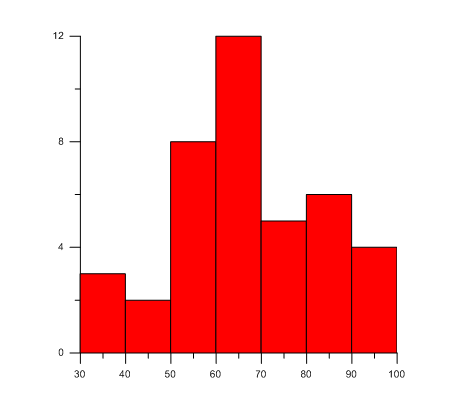
\includegraphics[scale=2]{images/histogram}
\caption{An example about histogram}
\label{fig:figure_31}
\end{figure}
\section{Segmentation}
Segmentation subdivides an image into its regions. The size of regions is depend on the problem being solved. This mean, segmentation should stop when the regions of interest in application have been detected. In the real, the segmentation was applied into many fields such as machine vision, medical imaging, object detection, etc. The most of segmentation algorithms are based on the basic properties of intensity values: discontinuity and similarity. In the first case, the segmentation based on abrupt changes in intensity. The second case, the image segmentation based on a predefined criteria. It means the image was segmented into regions that are similar according to a set of criteria. And, we have many the method to segment an image such as thresholding method, region growing, clustering method, histogram-based method, etc.\\[0.5 cm]
\textbf{Thresholding} is a simplest method of image segmentation. Thresholding use a particular threshold value ``t", we split the image into two parts: the first part includes pixels which have the value greater than t, and the second part contains the pixels vice versa. With this technique, thresholding can be used to create an binary image from a gray scale image. In fact, we have many type of threshold, as follows:
\begin{itemize}
\item \textit{Global thresholding}, when t is a constant over an entire image
\item \textit{Variable thresholding}, when t changes over an image
\item \textit{Local or regional thresholding}, is variable threshoding in a region of an image
\item \textit{Dynamic or adaptive thresholding}, if t depends on the spatial coordinates.
\item \textit{Multiple thresholding}, thresholding on 3 dominant modes (color image)
\end{itemize}
\section{Color processing}\label{color_model}
The use of color in image processing do not just identify or extract an objects from scene, it also a factor for image analysis.

